\documentclass[12pt]{article}
\usepackage[margin=2.5cm]{geometry}
\usepackage{enumerate}
\usepackage{amsfonts}
\usepackage{amsmath}
\usepackage{fancyhdr}
\usepackage{amsmath}
\usepackage{amssymb}
\usepackage{amsthm}
\usepackage{mdframed}
\usepackage{graphicx}
\usepackage{subcaption}
\usepackage{adjustbox}
\usepackage{listings}
\usepackage{xcolor}
\usepackage{booktabs}
\usepackage[utf]{kotex}
\usepackage{hyperref}

\definecolor{codegreen}{rgb}{0,0.6,0}
\definecolor{codegray}{rgb}{0.5,0.5,0.5}
\definecolor{codepurple}{rgb}{0.58,0,0.82}
\definecolor{backcolour}{rgb}{0.95,0.95,0.92}

\lstdefinestyle{mystyle}{
    backgroundcolor=\color{backcolour},
    commentstyle=\color{codegreen},
    keywordstyle=\color{magenta},
    numberstyle=\tiny\color{codegray},
    stringstyle=\color{codepurple},
    basicstyle=\ttfamily\footnotesize,
    breakatwhitespace=false,
    breaklines=true,
    captionpos=b,
    keepspaces=true,
    numbers=left,
    numbersep=5pt,
    showspaces=false,
    showstringspaces=false,
    showtabs=false,
    tabsize=1
}

\lstset{style=mystyle}

\pagestyle{fancy}
\renewcommand{\headrulewidth}{0.4pt}
\lhead{Hyungmo Gu}
\rhead{CSC369 Week 2 Notes}

\begin{document}
\title{CSC369 Week 2 Notes}
\author{Hyungmo Gu}
\maketitle

\section{System Calls}

\bigskip

\begin{itemize}
    \item Bootstraping
    \begin{itemize}
        \item \textbf{Bootstrap Program:} is the first code that is executed when
        the computer system is started
        \item Entires operating system depnds on the bootstrap program to work
        correctly

        \item Bootstrap program is loaded onto ROM

        \begin{center}
        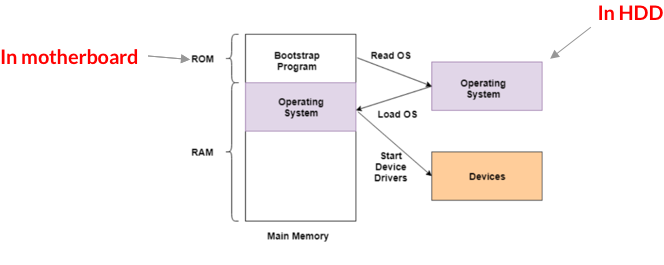
\includegraphics[width=\linewidth]{images/week_2_notes_1_1.png}
        \end{center}

        \begin{itemize}
            \item ROM is called \textbf{read-only-memory}
            \item Is also called \textbf{BIOS chip} (Basic Input/Output System)
            \item ROM is non-volatile memory
            \item ROM is stored in motherboard
        \end{itemize}

        \item Knows how to access simple hardware devices
        \begin{itemize}
            \item i.e. Disk, keyboard, display
        \end{itemize}

        \begin{center}
        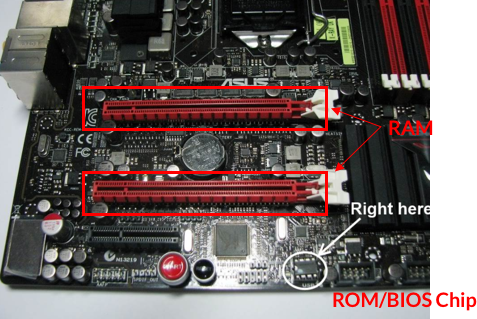
\includegraphics[width=0.8\linewidth]{images/week_2_notes_1_2.png}
        \end{center}

    \end{itemize}
\end{itemize}

\end{document}